\begin{figure*}[htbp]
     \centering
     % First Row
     \begin{subfigure}[b]{0.49\textwidth}
         \centering
         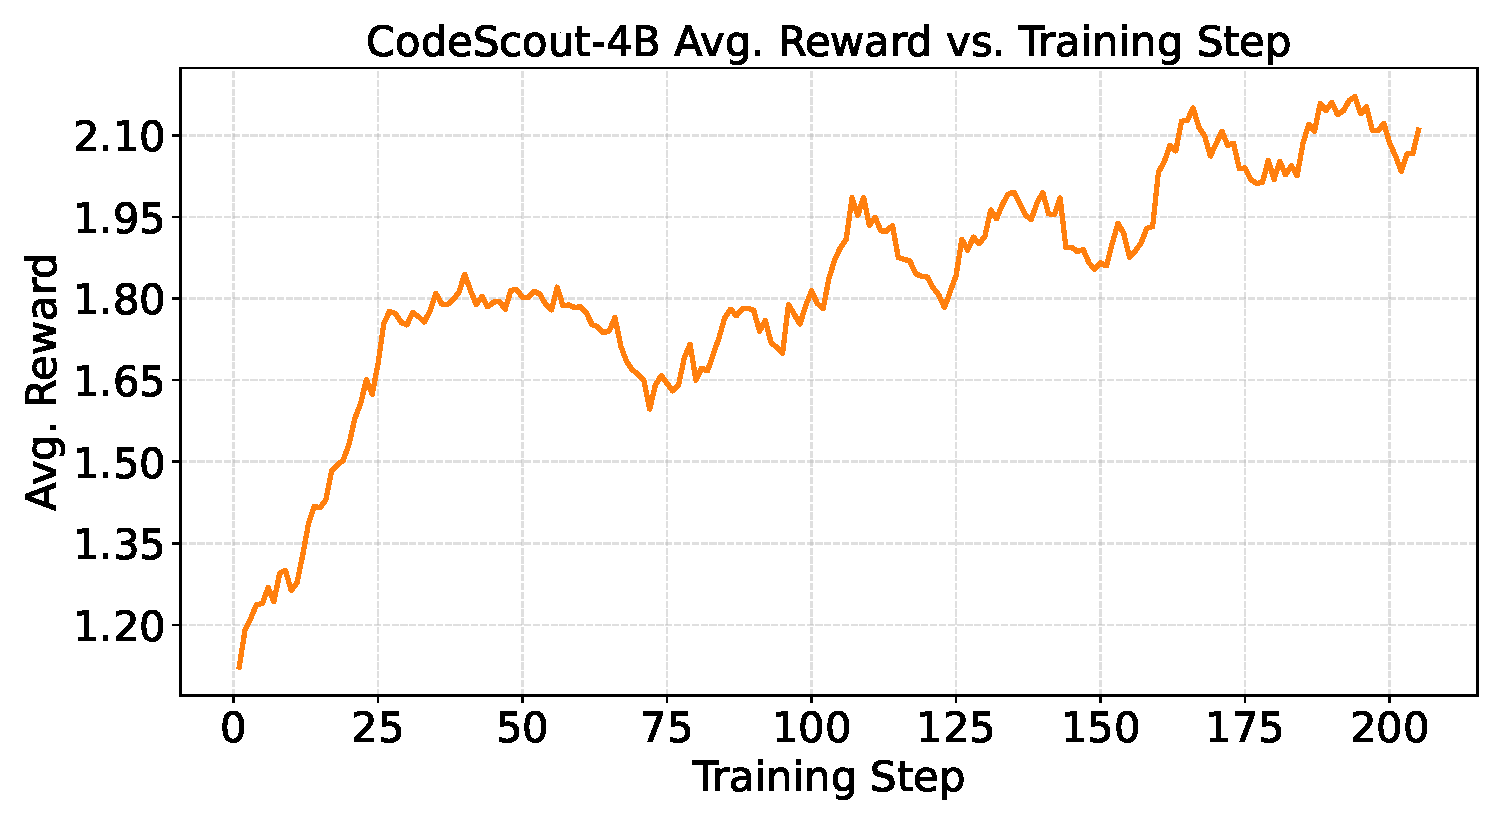
\includegraphics[width=\textwidth]{Figures/codescout_4b/4B_all_reward_curve.pdf}
         \caption{Aggregate reward vs. Training Step}
         \label{fig:codescout_4b_avg}
     \end{subfigure}
     \hfill
     \begin{subfigure}[b]{0.49\textwidth}
         \centering
         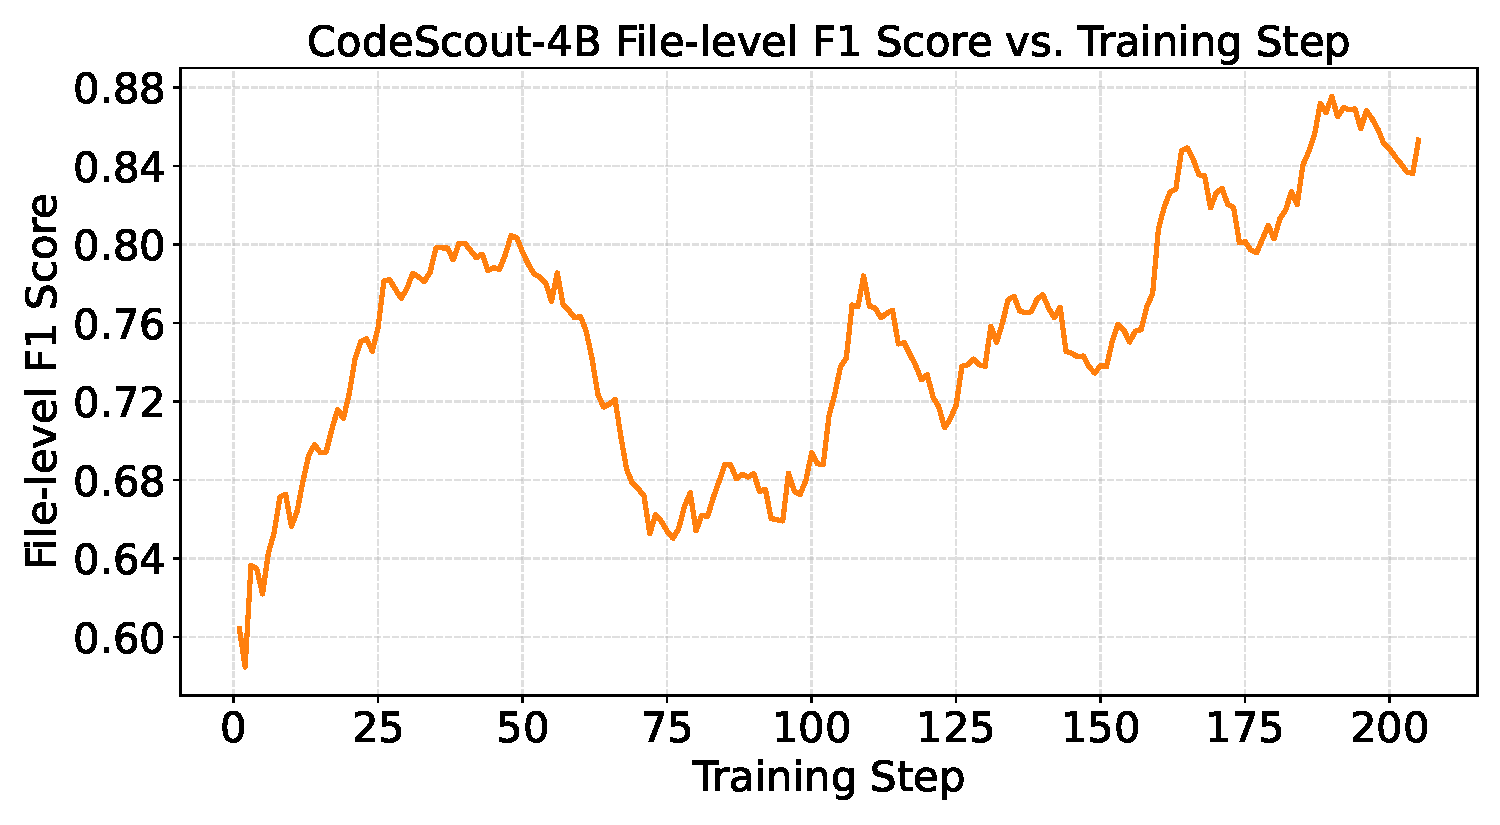
\includegraphics[width=\textwidth]{Figures/codescout_4b/4B_file_reward_curve.pdf}
         \caption{File-level F1 score vs. Training Step}
         \label{fig:image2}
     \end{subfigure}

    %  \vspace{5pt} % Adds vertical space between the rows

     % Second Row
     \begin{subfigure}[b]{0.49\textwidth}
         \centering
         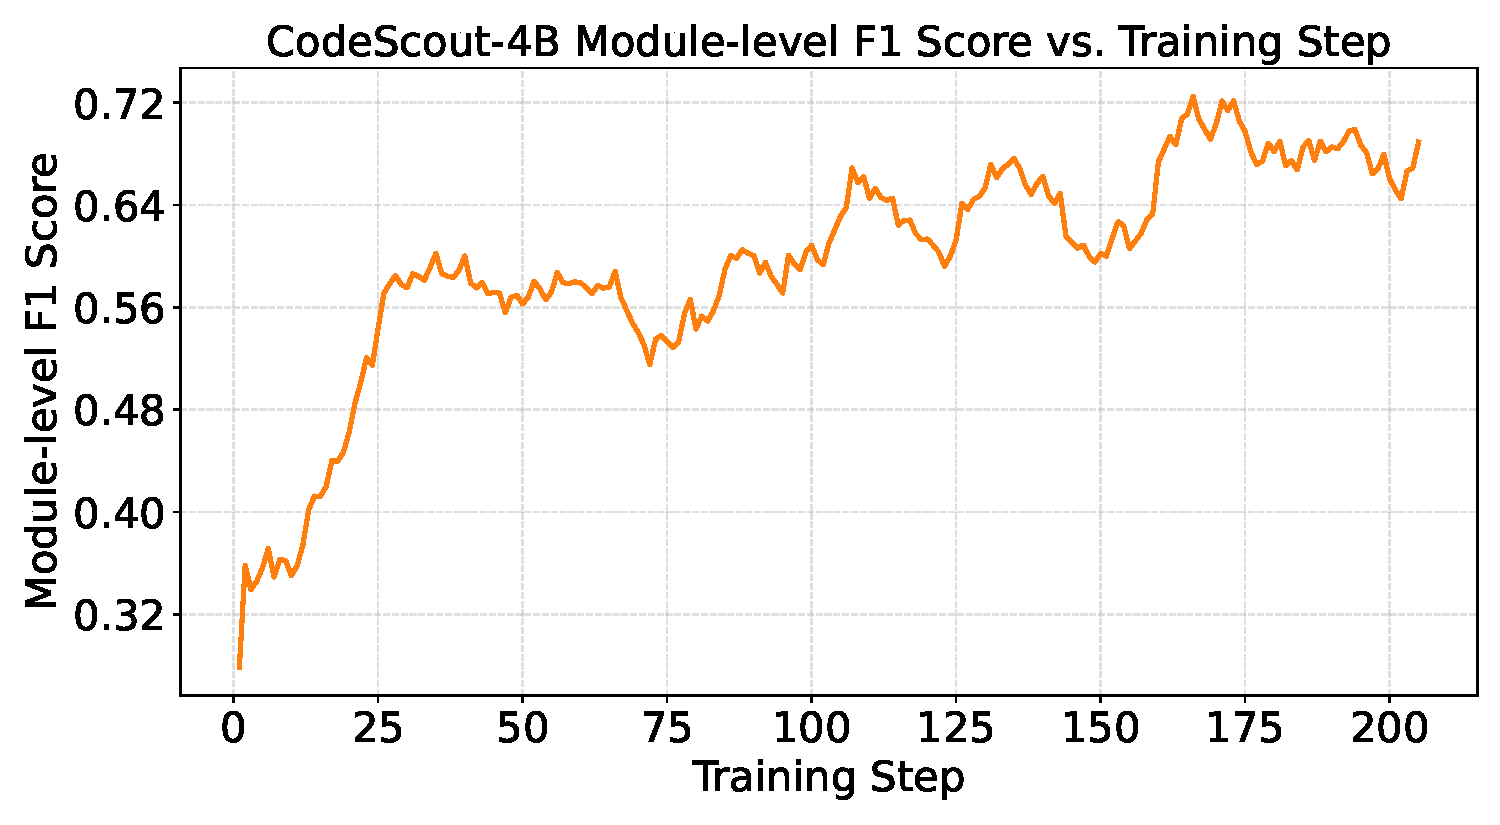
\includegraphics[width=\textwidth]{Figures/codescout_4b/4B_module_reward_curve.pdf}
         \caption{Module-level F1 score vs. Training Step}
         \label{fig:image3}
     \end{subfigure}
     \hfill
     \begin{subfigure}[b]{0.49\textwidth}
         \centering
         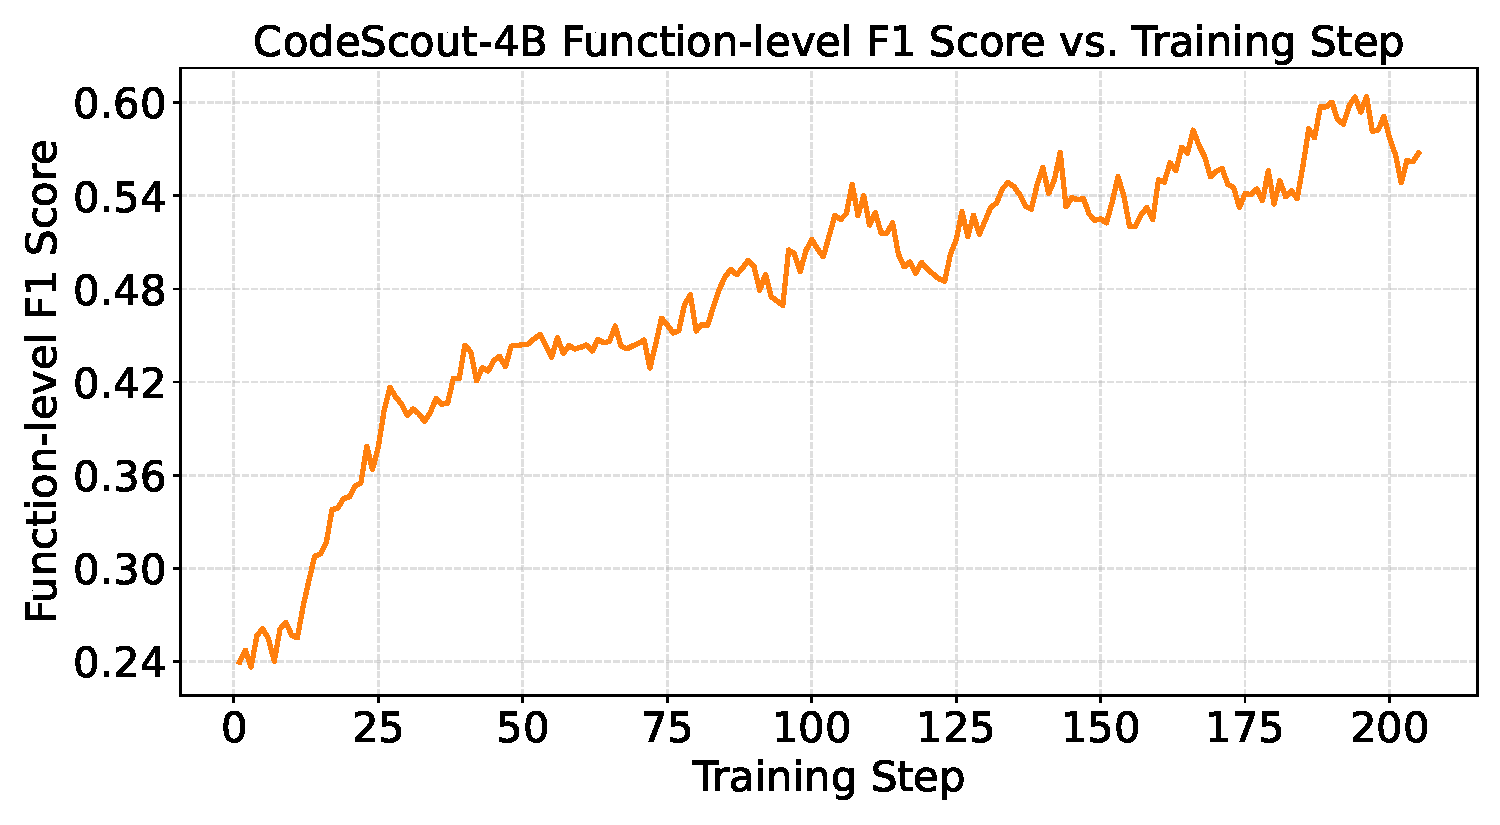
\includegraphics[width=\textwidth]{Figures/codescout_4b/4B_function_reward_curve.pdf}
         \caption{Function-level F1 score vs. Training Step}
         \label{fig:image4}
     \end{subfigure}
     
     \caption{Reward curves for RL training of \methodname-4B.}
     \label{fig:codescout_4b_reward}
     \Description{Four subfigures showing the reward curves for RL training of CodeScout-4B - aggregate reward, file-level F1 score, module-level F1 score, and function-level F1 score plotted against training steps.}
\end{figure*}